\chapter{Mixing, Oscillation, Electric Dipole Moments, and Field Operators}

This chapter follows Leonard Susskind's \emph{Advanced Quantum Mechanics} Lecture 8 and is curated by LazyingArt LLC. It begins with a student question about neutrinos and energy conservation, turns that question into a concrete two-state problem in a symmetric double well, pauses for a deliberate interlude on the electric dipole moment of the electron, and then returns to second quantization. The thread that holds the lecture together is the distinction between the states in which systems are prepared and the states that diagonalize the Hamiltonian. Once that distinction is kept in view, mixing, oscillation, symmetry arguments, and field-operator commutators all become much more transparent.

\section{Mixing as the Real Issue}

The lecture opens with a question from particle physics: if neutrinos have different masses, how can they mix without violating energy conservation? Susskind's answer comes before any detailed mathematics. Energy eigenstates do not mix with one another. What mixes are the states used to describe \emph{type}: electron neutrino, muon neutrino, left well, right well, spin up, spin down. Schematically,
\begin{equation}
|\text{type}\rangle = \sum_n c_n |E_n\rangle.
\end{equation}
The right way to think is therefore not that energy conservation fails, but that the physically named states need not be eigenstates of energy.

To make this visible, Susskind immediately turns to a one-dimensional symmetric double-well potential with a high barrier between the wells. If the barrier were literally infinite, one could treat the two sides independently. Then there would be an approximate left-localized ground state and an approximate right-localized ground state, each with the same energy \(E\). In each single well the ground-state wavefunction is smooth and has no node.

\begin{figure}
\centering
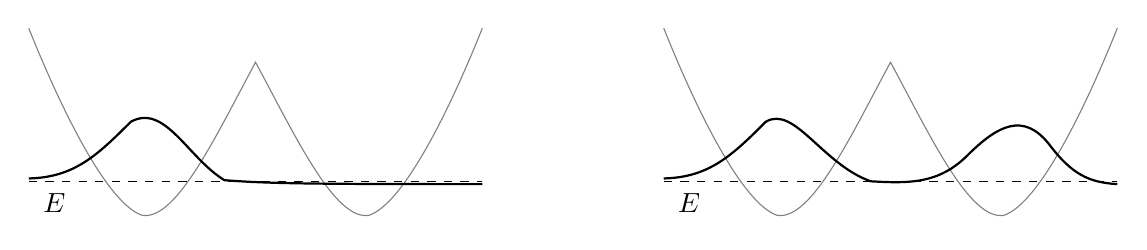
\begin{tikzpicture}[x=0.72cm,y=0.72cm]
\begin{scope}[shift={(-5.6,0)}]
\draw[gray] (-4,2.6) .. controls (-3.4,1.1) and (-2.6,-0.5) .. (-2.0,-0.7)
           .. controls (-1.4,-0.8) and (-0.7,0.7) .. (0,2.0)
           .. controls (0.7,0.7) and (1.4,-0.8) .. (2.0,-0.7)
           .. controls (2.6,-0.5) and (3.4,1.1) .. (4,2.6);
\draw[dashed] (-4,-0.10) -- (4,-0.10);
\node at (-3.55,-0.48) {$E$};
\draw[thick] (-4,-0.05) .. controls (-3.2,-0.03) and (-2.8,0.35) .. (-2.2,0.95)
             .. controls (-1.6,1.28) and (-1.2,0.32) .. (-0.55,-0.08)
             .. controls (0.2,-0.14) and (1.0,-0.15) .. (4,-0.15);
\end{scope}
\begin{scope}[shift={(5.6,0)}]
\draw[gray] (-4,2.6) .. controls (-3.4,1.1) and (-2.6,-0.5) .. (-2.0,-0.7)
           .. controls (-1.4,-0.8) and (-0.7,0.7) .. (0,2.0)
           .. controls (0.7,0.7) and (1.4,-0.8) .. (2.0,-0.7)
           .. controls (2.6,-0.5) and (3.4,1.1) .. (4,2.6);
\draw[dashed] (-4,-0.10) -- (4,-0.10);
\node at (-3.55,-0.48) {$E$};
\draw[thick] (-4,-0.05) .. controls (-3.2,-0.03) and (-2.8,0.35) .. (-2.2,0.95)
             .. controls (-1.7,1.25) and (-1.2,0.20) .. (-0.35,-0.10)
             .. controls (0.35,-0.14) and (0.85,-0.14) .. (1.35,0.35)
             .. controls (1.9,0.90) and (2.35,1.12) .. (2.80,0.55)
             .. controls (3.20,0.02) and (3.50,-0.12) .. (4,-0.15);
\end{scope}
\end{tikzpicture}
\caption{A schematic version of the board sketches. On the left is a left-localized trial state in a high barrier double well. On the right is the symmetrically continued state which anticipates the true even ground state. The essential feature is the small but nonzero amplitude in the barrier region.}
\end{figure}

But the barrier is not truly infinite. Quantum mechanically there is a small tunneling amplitude, so the wavefunction in the barrier region is tiny, but not exactly zero. This tiny leakage is the origin of the splitting.

\section{Parity Eigenstates and the Split Spectrum}

The crucial correction to the naive left-right picture comes from symmetry.

\begin{theorem}
If the one-dimensional potential satisfies \(V(x)=V(-x)\), then the energy eigenfunctions may be chosen to be either even or odd under reflection.
\end{theorem}

The localized trial functions are neither even nor odd, so they cannot be exact eigenstates of the full Hamiltonian. The correct energy eigenstates are instead the symmetric and antisymmetric combinations
\begin{align}
\psi_+ &= \frac{\psi_L+\psi_R}{\sqrt{2}},\\
\psi_- &= \frac{\psi_L-\psi_R}{\sqrt{2}}.
\end{align}
The board notation then assigns to these states slightly different energies:
\begin{align}
H\psi_+ &= (E_1-\epsilon)\psi_+,\\
H\psi_- &= (E_1+\epsilon)\psi_-.
\end{align}

Here \(\epsilon\) is half the energy splitting. Susskind emphasizes two qualitative points.

First, the symmetric state is slightly lower in energy. The reason is not mysterious: it is smoother through the barrier region. One can lower the energy by allowing the wavefunction to leak a little and continue symmetrically across the midpoint.

Second, the antisymmetric state is slightly higher in energy. In a symmetric one-dimensional problem the first excited state has one node, and the odd combination has precisely such a node at the center. More curvature means higher kinetic energy, and so the antisymmetric state is pushed upward.

The splitting is small, indeed exponentially small in the barrier parameters. Susskind does not compute \(\epsilon\) in detail, but he stresses that it is extremely sensitive to the mass, the width of the barrier, and the barrier height.

An overall sign of an eigenfunction is physically immaterial. In particular, replacing \(\psi_-\) by \(-\psi_-\) changes nothing. What matters is the parity and the energy.

\section{Time Evolution and Left-Right Oscillation}

Once the spectrum has been reorganized into exact eigenstates, the lecture turns to the dynamical question: what happens if a particle is initially placed in the left well?

At \(t=0\) the initial state is
\begin{equation}
\psi(0)=\psi_L=\frac{\psi_+ + \psi_-}{\sqrt{2}}.
\end{equation}
This is not an energy eigenstate, so its time dependence is nontrivial.

\begin{remark}
On the board the signs in the time-dependent phases wobble for a moment, and Susskind explicitly notices the slip. The robust content is the relative phase between the two energy eigenstates, so in the written notes it is best to adopt the standard Schr\"odinger convention \(e^{-iEt}\).
\end{remark}

The time-evolved state is therefore
\begin{align}
\psi(t)
&= \frac{1}{\sqrt{2}}\left(e^{-i(E_1-\epsilon)t}\psi_+ + e^{-i(E_1+\epsilon)t}\psi_-\right) \\
&= \frac{e^{-iE_1 t}}{\sqrt{2}}\left(e^{i\epsilon t}\psi_+ + e^{-i\epsilon t}\psi_-\right).
\end{align}
Now substitute back
\[
\psi_+ = \frac{\psi_L+\psi_R}{\sqrt{2}},
\qquad
\psi_- = \frac{\psi_L-\psi_R}{\sqrt{2}},
\]
to obtain the localized-basis form
\begin{align}
\psi(t)
&= e^{-iE_1 t}\left[\psi_L\cos(\epsilon t) + i\,\psi_R\sin(\epsilon t)\right].
\end{align}
In the two-state approximation, where \(\psi_L\) and \(\psi_R\) are taken orthonormal, the probabilities are
\begin{equation}
P_L(t)=\cos^2(\epsilon t),
\qquad
P_R(t)=\sin^2(\epsilon t).
\end{equation}
Thus the particle oscillates from one side to the other. The probability oscillation has period \(\pi/\epsilon\), and after one half of that probability period the particle has transferred from left to right.

Susskind writes the transfer condition on the board as a statement about the relative phase:
\begin{equation}
e^{-i\epsilon t}=-e^{i\epsilon t}
\qquad \Longleftrightarrow \qquad
e^{2i\epsilon t}=-1.
\end{equation}
The first time this happens is when
\begin{equation}
2\epsilon t=\pi,
\qquad\text{so that}\qquad
t_{L\to R}=\frac{\pi}{2\epsilon}.
\end{equation}
At that moment the state is proportional to \(\psi_R\):
\begin{equation}
\psi\!\left(\frac{\pi}{2\epsilon}\right)
= i\,e^{-iE_1\pi/(2\epsilon)}\psi_R.
\end{equation}
The overall phase is unobservable. What matters is that a particle initially localized on the left has evolved into a state localized on the right.

Susskind makes one verbal slip a few moments later and says that small \(\epsilon\) makes the transfer time small. The derived formula says the opposite: small \(\epsilon\) means a long transfer time, which is physically the correct statement.

The main moral is that mixing and oscillation are not two separate phenomena. They are the static and dynamic faces of the same two-state system.

\section{Neutrino and Spin Analogies}

With the double-well calculation in place, Susskind returns to the neutrino question. In the lecture's simplified two-state picture, the flavor states play the role of the localized states, while the mass or energy eigenstates play the role of \(\psi_\pm\). Schematically,
\begin{align}
|\nu_e\rangle &= \frac{|m_+\rangle + |m_-\rangle}{\sqrt{2}},\\
|\nu_\mu\rangle &= \frac{|m_+\rangle - |m_-\rangle}{\sqrt{2}}.
\end{align}
A neutrino produced in association with an electron is created in the ``electron-neutrino'' state, just as a particle can be placed in the left well. But the Hamiltonian evolves the mass eigenstates independently, not the flavor states. Relative phases accumulate, and after a sufficiently long baseline an electron neutrino can behave as a muon neutrino.

This is the lecture's qualitative picture of long-baseline oscillation and of the solar-neutrino deficit: by the time neutrinos arrive, some of the original electron-type neutrinos have converted into other types and no longer interact as electron neutrinos.

Susskind also discusses ammonia inversion. There the same mathematics appears in a molecular setting: the nitrogen can tunnel from one side of the hydrogen plane to the other, producing symmetric and antisymmetric combinations. The neutrino problem is not a spatial tunneling problem in the same literal sense, but the algebra is the same because in both cases there is an off-diagonal coupling in the Hamiltonian.

\paragraph{Spin in a weak magnetic field.}
To show that no physical barrier is required, Susskind turns to spin. Begin with the \(z\)-basis states \(|\uparrow_z\rangle\) and \(|\downarrow_z\rangle\). If a weak magnetic field points along the \(x\)-axis, then the energy eigenstates are the \(x\)-polarized states, which he temporarily calls left and right:
\begin{align}
|L_x\rangle &= \frac{|\uparrow_z\rangle + |\downarrow_z\rangle}{\sqrt{2}},\\
|R_x\rangle &= \frac{|\uparrow_z\rangle - |\downarrow_z\rangle}{\sqrt{2}}.
\end{align}
These are the direct analogues of \(\psi_+\) and \(\psi_-\), and they acquire slightly different phases because the field splits their energies.

If one begins with \(|\uparrow_z\rangle\), then the state is again a superposition of exact energy eigenstates. The same two-state algebra leads to oscillation. Susskind describes it in physical language as precession: after a half period the spin is found down, after another half period it returns up. The field need only be weak if one wants the oscillation to be slow. The weakness of the field changes the period, not the mechanism.

The neutrino, double-well, ammonia, and spin examples are all instances of the same structure: a prepared state is not an energy eigenstate, and the relative phases of the true eigenstates eventually change what the prepared state looks like.

\section{Interlude: Electric Dipole Moments and the Question of Shape}

Susskind then takes a deliberate break from formal quantum field theory and discusses a popular claim that a null measurement of the electron's electric dipole moment shows that ``the electron is a sphere.'' His point is that this is a category mistake.

\subsection{What an electric dipole moment means}

\begin{definition}
For a pair of opposite charges \(\pm q\) separated by a vector \(\vec{\ell}\), the electric dipole moment is
\begin{equation}
\vec d = q\,\vec{\ell}.
\end{equation}
\end{definition}

An electric dipole moment is therefore evidence of an off-centered charge distribution. But the absence of a dipole moment does \emph{not} imply spherical symmetry. A charge distribution can have no dipole moment and still have quadrupole or higher multipole moments. An ellipsoid, for example, can have zero dipole moment and yet not be a sphere.

For the electron the relevant question is more specific. The electron has spin, and hence an axis. Relative to that axis, is there a displacement of charge? If so, one would say that the electron has an electric dipole moment aligned with its spin or magnetic axis.

Idealized energetically, the measurement would look like the familiar dipole energy shift:
\begin{equation}
\Delta E_{\text{mag}} = - \vec{\mu}_e \cdot \vec B,
\qquad
\Delta E_{\text{elec}} = - \vec d_e \cdot \vec E.
\end{equation}
The practical experiment is much more subtle than this elementary formula, but this is the conceptual core: does an electric field split the two spin orientations because the electron carries an EDM?

\subsection{Why ``no EDM'' does not mean ``sphere''}

Susskind next discusses a quantum mechanical dumbbell. Even a lopsided object can have a rotationally invariant \emph{ground state}. For a bosonic rotor the ground state has angular momentum \(J=0\), and since angular momentum generates rotations, a \(J=0\) state is rotationally symmetric. Thus the wavefunction can be spherically symmetric even when the underlying classical picture is elongated.

This does not mean the object has become classically spherical. It means that the ground state is a superposition of orientations. A sufficiently sharp measurement of orientation would collapse the state into a definite orientation and thereby disturb its angular momentum. Susskind presents this as the angular analogue of the usual position-momentum story: measuring orientation gives a kick to angular momentum.

The practical moral is that ``shape'' in quantum mechanics depends on the probe. If the first excited rotational state lies extremely close to the ground state, an ordinary measurement can resolve the orientation. If the excitation gap is extremely large, then ordinary low-energy probes only see the rotationally averaged state. This is part of the reason why he treats the word ``sphere'' with suspicion.

He then makes an even simpler point about the electron. Independently of any EDM measurement, the electron is not a featureless scalar object. It has spin and therefore has an axis. It has a magnetic moment and therefore a preferred orientation. In that ordinary sense alone, it is already misleading to call the electron ``a sphere.''

\subsection{Parity and time reversal}

The deeper content of the EDM discussion is symmetry. The electric dipole moment and the magnetic moment transform differently under parity and time reversal. In the cleaned notation,
\begin{align}
P:\qquad &\vec d_e \to -\vec d_e,
&\vec \mu_e \to \vec \mu_e,\\
T:\qquad &\vec d_e \to \vec d_e,
&\vec \mu_e \to -\vec \mu_e.
\end{align}
So a nonzero EDM aligned with the electron's magnetic axis would violate parity, and it would also violate time reversal.

Susskind's verbal argument is geometric. Under mirror reflection, a magnetic moment behaves like an axial vector and keeps its direction, while the displacement of charge behaves like an ordinary polar vector and flips. If there is only one species of electron and parity is exact, the mirror image must describe the same electron. The only way this can happen is for the charge to remain centered, so that \(\vec d_e=0\).

Time reversal leads to the same conclusion in a different way. Under reversal of the movie, the circulating current that defines the magnetic moment reverses, so the magnetic axis flips. But the static electric displacement does not reverse. Again, if the time-reversed object is to be the same electron, the only consistent possibility is zero EDM.

In compact form,
\begin{equation}
(P\ \text{exact}) \Rightarrow \vec d_e = 0,
\qquad
(T\ \text{exact}) \Rightarrow \vec d_e = 0.
\end{equation}

Now the world is not parity invariant; weak interactions violate parity strongly. Time reversal is also not exact. But time-reversal violation in the standard model is tiny, and therefore the standard-model prediction for the electron EDM is extremely small. The experiment Susskind is discussing measured no EDM. That is good news for the standard model and bad news for many speculative extensions, because it removes available room for additional \(T\)-violating interactions.

So the lesson of the interlude is not that the electron is spherical. The lesson is that a null EDM measurement is a symmetry statement and a constraint on possible modifications of the standard model.

\section{Return to Second Quantization: Fourier Transforms, Modes, and Locality}

After the break Susskind explicitly returns to the main course thread: second quantization. He begins again from something familiar, namely the ordinary Fourier transform of a one-particle wavefunction.

\subsection{One-particle wavefunctions and their Fourier transforms}

Let \(\psi(x)\) be the wavefunction of a single particle in position space. Then
\begin{equation}
P(x)=|\psi(x)|^2
\end{equation}
is the probability density for finding the particle at position \(x\). The momentum-space wavefunction is its Fourier transform,
\begin{equation}
\tilde{\psi}(p)=\int dx\,\psi(x)\,\frac{e^{-ipx}}{\sqrt{2\pi}},
\end{equation}
and the inverse transform is
\begin{equation}
\psi(x)=\int dp\,\tilde{\psi}(p)\,\frac{e^{ipx}}{\sqrt{2\pi}}.
\end{equation}
Then
\begin{equation}
P(p)=|\tilde{\psi}(p)|^2
\end{equation}
is the probability density for momentum \(p\).

For a free particle,
\begin{equation}
H=\frac{p^2}{2m},
\end{equation}
so momentum eigenstates are automatically energy eigenstates, and their position-space wavefunctions are plane waves,
\begin{equation}
\psi_p(x)\propto e^{ipx}.
\end{equation}

\subsection{From amplitudes to operators}

Susskind then lifts this structure into second quantization. On the board he writes the annihilation and creation pieces as \(\Psi_-(x)\) and \(\Psi_+(x)\). In the notes it is convenient to use the more standard notation \(\Psi(x)\) and \(\Psi^\dagger(x)\), while keeping exactly the same logic.

For a discrete orthonormal basis of one-particle states \(\{\psi_i(x)\}\),
\begin{align}
\Psi(x) &= \sum_i a_i\,\psi_i(x),\\
\Psi^\dagger(x) &= \sum_i a_i^\dagger\,\psi_i^*(x).
\end{align}
Here \(a_i\) annihilates a particle in the \(i\)-th mode and \(a_i^\dagger\) creates one.

In the free-particle momentum basis, sums become integrals. Since the one-particle eigenfunctions are plane waves, the field operator becomes
\begin{align}
\Psi(x) &= \int \frac{dp}{\sqrt{2\pi}}\,a(p)\,e^{ipx},\\
\Psi^\dagger(x) &= \int \frac{dp}{\sqrt{2\pi}}\,a^\dagger(p)\,e^{-ipx}.
\end{align}
These formulas invert exactly as Fourier transforms do:
\begin{align}
a(p) &= \int \frac{dx}{\sqrt{2\pi}}\,\Psi(x)\,e^{-ipx},\\
a^\dagger(p) &= \int \frac{dx}{\sqrt{2\pi}}\,\Psi^\dagger(x)\,e^{ipx}.
\end{align}

This is one of the central mathematical points of the second half of the lecture. In ordinary quantum mechanics, \(\psi(x)\) and \(\tilde{\psi}(p)\) are Fourier transforms of one another. In second quantization, the same relation reappears between the operator that creates or annihilates a particle at a point and the operator that creates or annihilates a particle with a definite momentum.

Thus \(\Psi^\dagger(x)\) creates a particle localized at position \(x\), while \(a^\dagger(p)\) creates a particle with momentum \(p\). Position-space and momentum-space creation operators are Fourier conjugates.

\subsection{Bosonic commutators and the meaning of locality}

For bosons the creation and annihilation operators satisfy
\begin{equation}
[a_i,a_j^\dagger]=\delta_{ij},
\qquad
[a_i,a_j]=0,
\qquad
[a_i^\dagger,a_j^\dagger]=0.
\end{equation}
Using the field expansion, one immediately obtains the equal-time field commutator:
\begin{align}
[\Psi(x),\Psi^\dagger(y)]
&= \sum_{i,j}\psi_i(x)\psi_j^*(y)\,[a_i,a_j^\dagger] \\
&= \sum_i \psi_i(x)\psi_i^*(y) \\
&= \delta(x-y).
\end{align}
Likewise,
\begin{equation}
[\Psi(x),\Psi(y)]=[\Psi^\dagger(x),\Psi^\dagger(y)]=0.
\end{equation}

Susskind's interpretation is very physical. The important fact is not primarily that \(\Psi(x)\) is non-Hermitian; one can always take real and imaginary parts. The important fact is the delta function. When \(x\neq y\), the fields commute, so measurements at separated points do not interfere with one another. When \(x=y\), the commutator is singular, meaning that the same-point real and imaginary parts cannot be measured simultaneously without mutual disturbance.

This is the lecture's bosonic locality heuristic. Degrees of freedom at different points behave independently, and that matches the basic intuition that measuring the field here should not instantly kick the field there. Susskind briefly pushes the point toward relativity and causality, and then uses it to set up the next lecture: fermions will require anti-commutators, and because fermion fields are not observables in the same direct sense, the story has to be told more carefully.

\section{Summary}

The lecture begins with a live particle-physics question and answers it by stripping away the misleading language of ``mixing energies.'' In the double well, the approximate localized states are not exact eigenstates. The true energy eigenstates are the even and odd combinations, split by a tiny tunneling effect. Once the system is prepared in a localized state, the relative phase of the exact eigenstates drives oscillation from left to right.

That same two-state structure then reappears in neutrino flavor change, ammonia inversion, and spin precession in a weak transverse magnetic field. The long interlude on the electron EDM serves a different purpose: it clarifies what symmetry arguments really say, and what they do \emph{not} say, about the shape of the electron. Finally, the lecture returns to second quantization, where Fourier transforms connect position-space and momentum-space field operators, and equal-time bosonic commutators express the independence of measurements at separated points. The next step, explicitly postponed to the following lecture, is the fermionic version of the same operator story.